\begin{figure}[!t]
\begin{tabular}{c c}
    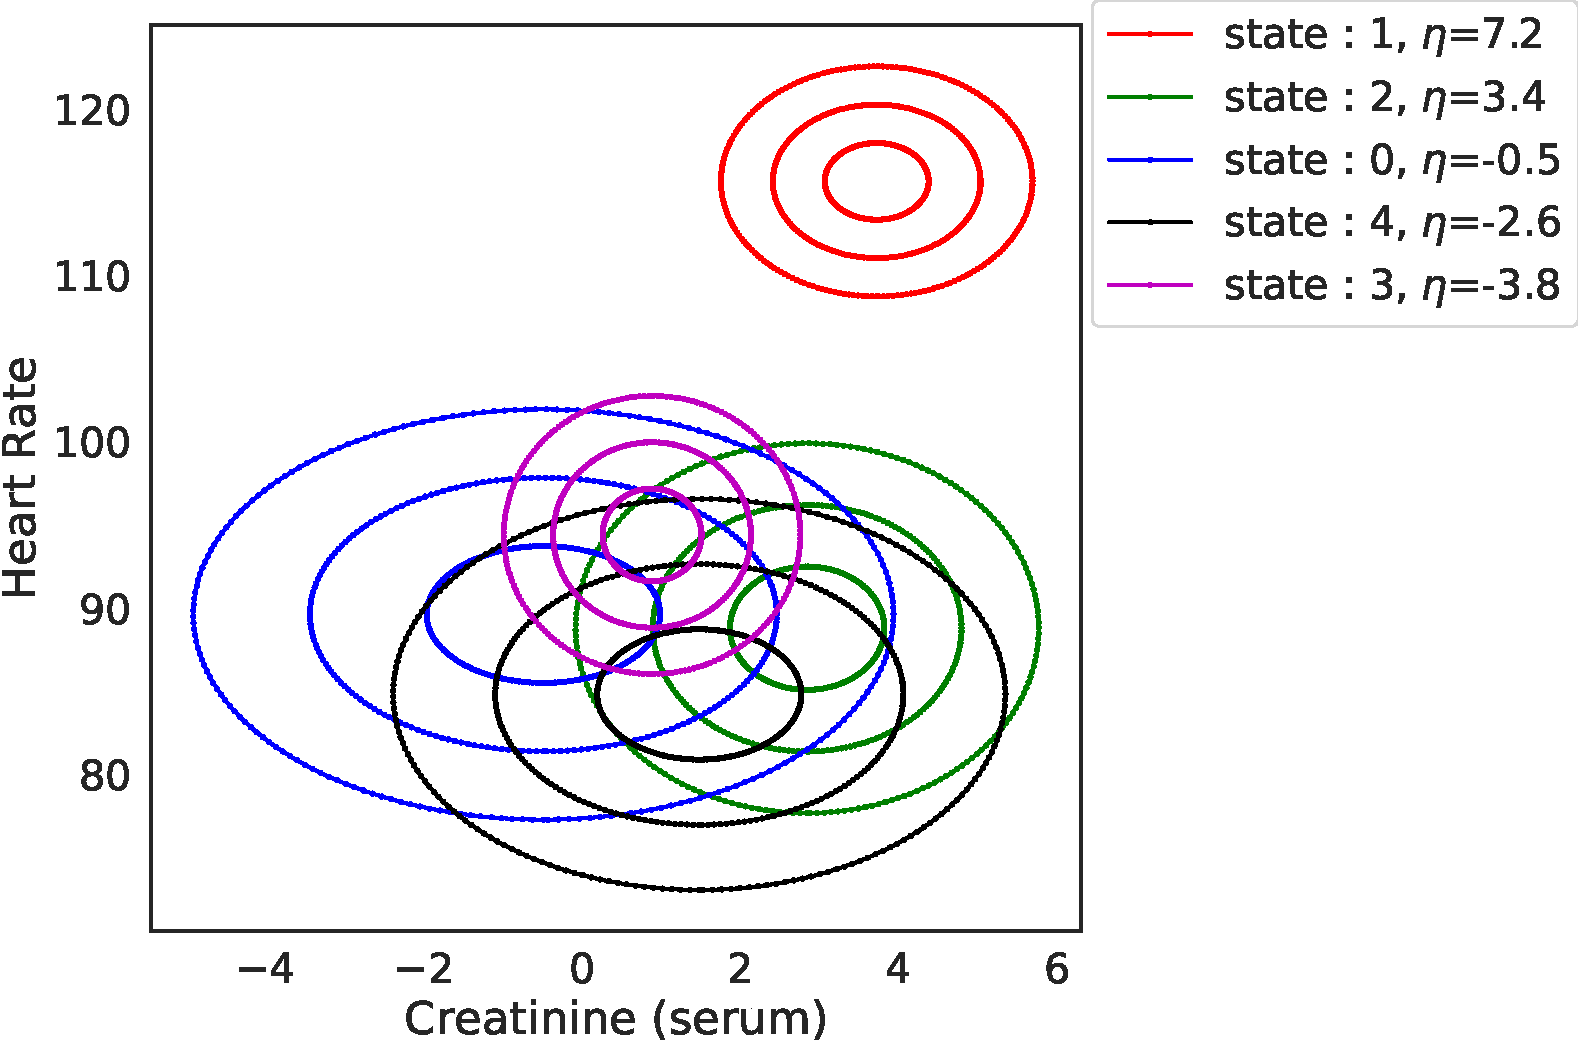
\includegraphics[width=0.5\textwidth]{content/chapters/semi_supervised_pchmm_missing_data/images/interpretability_Heart Rate_Creatinine (serum)_MIMIC.pdf} 
    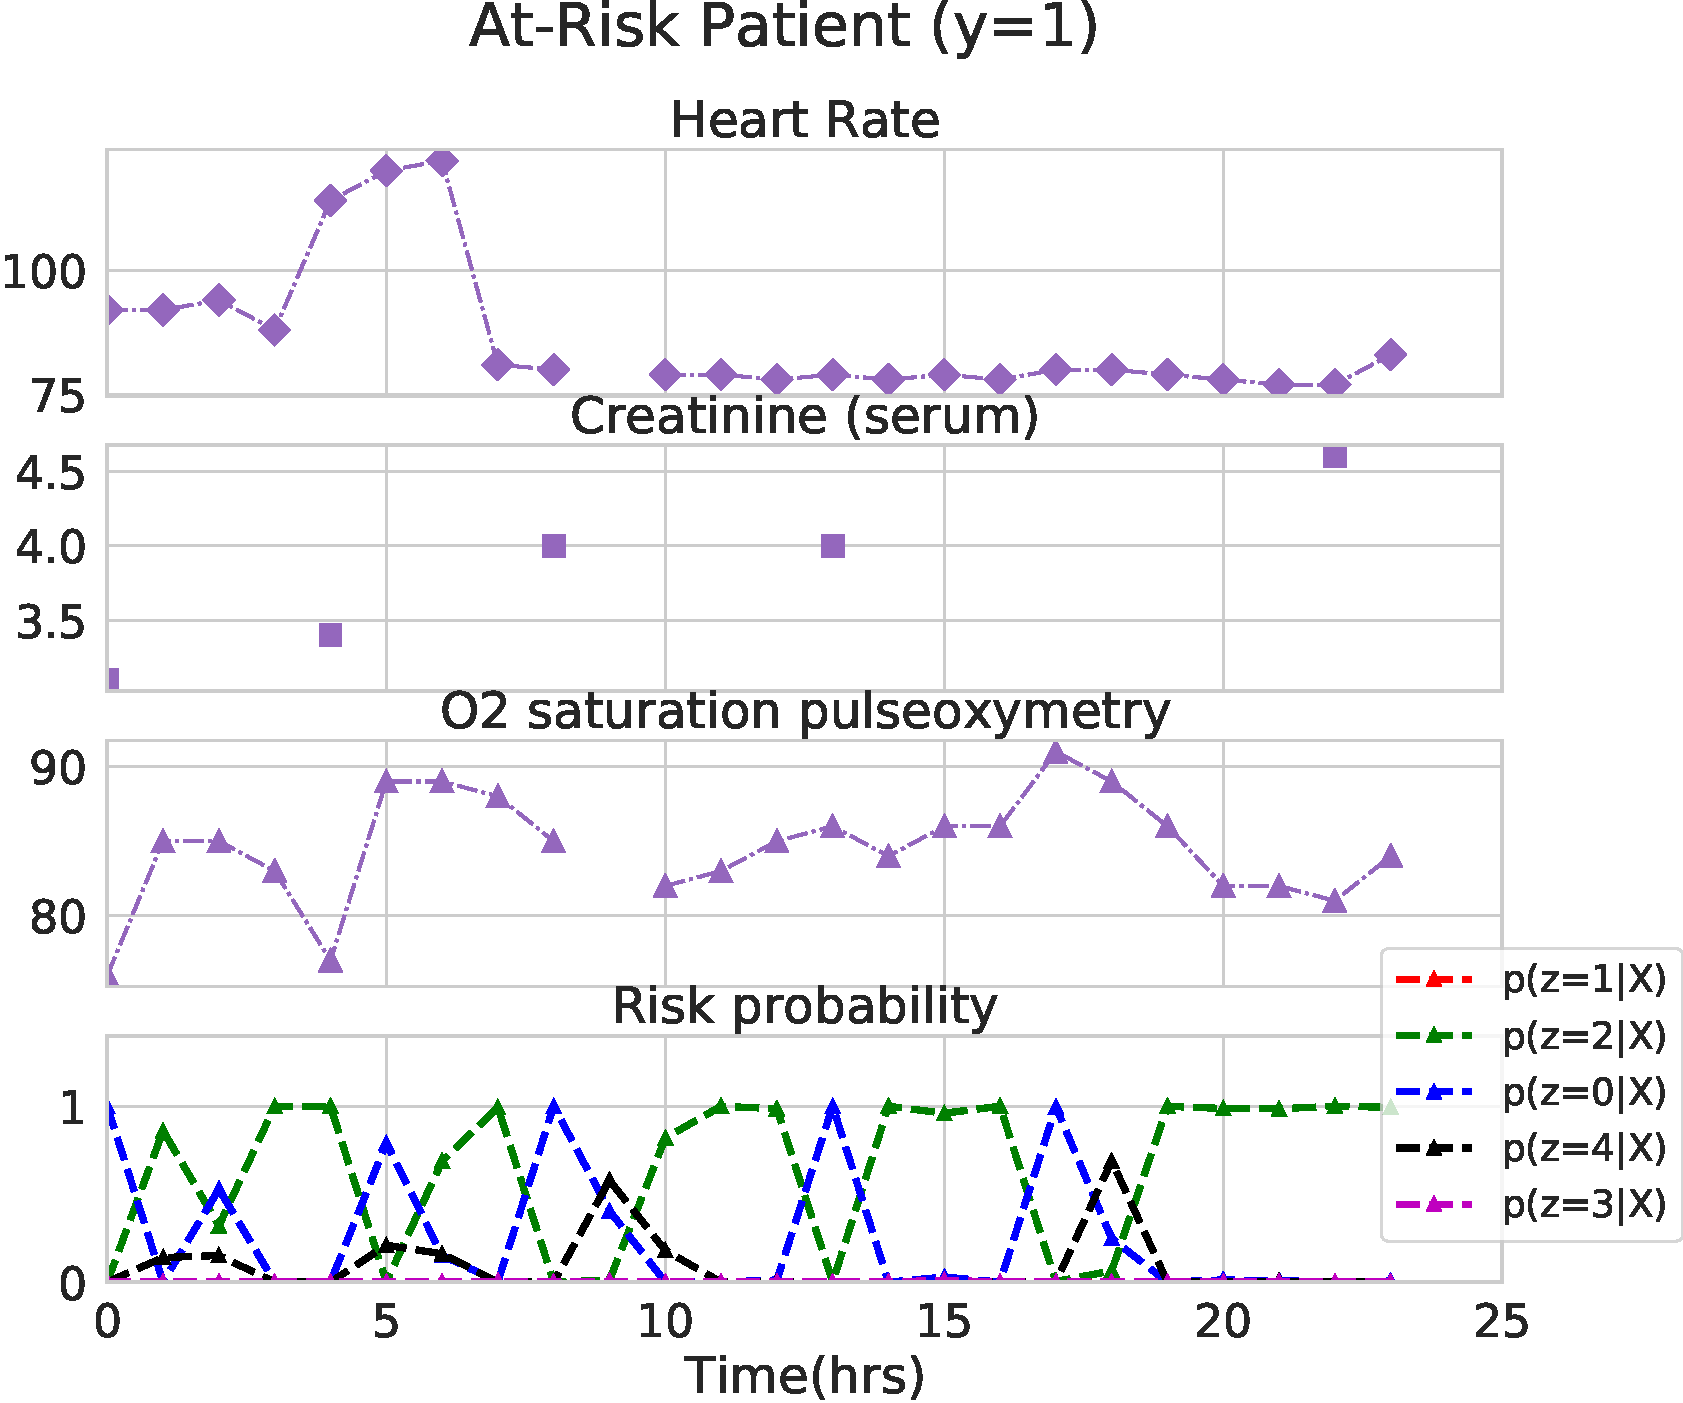
\includegraphics[width=0.5\textwidth]{content/chapters/semi_supervised_pchmm_missing_data/images/mortality_risk_patient_interpretability.pdf} \\
    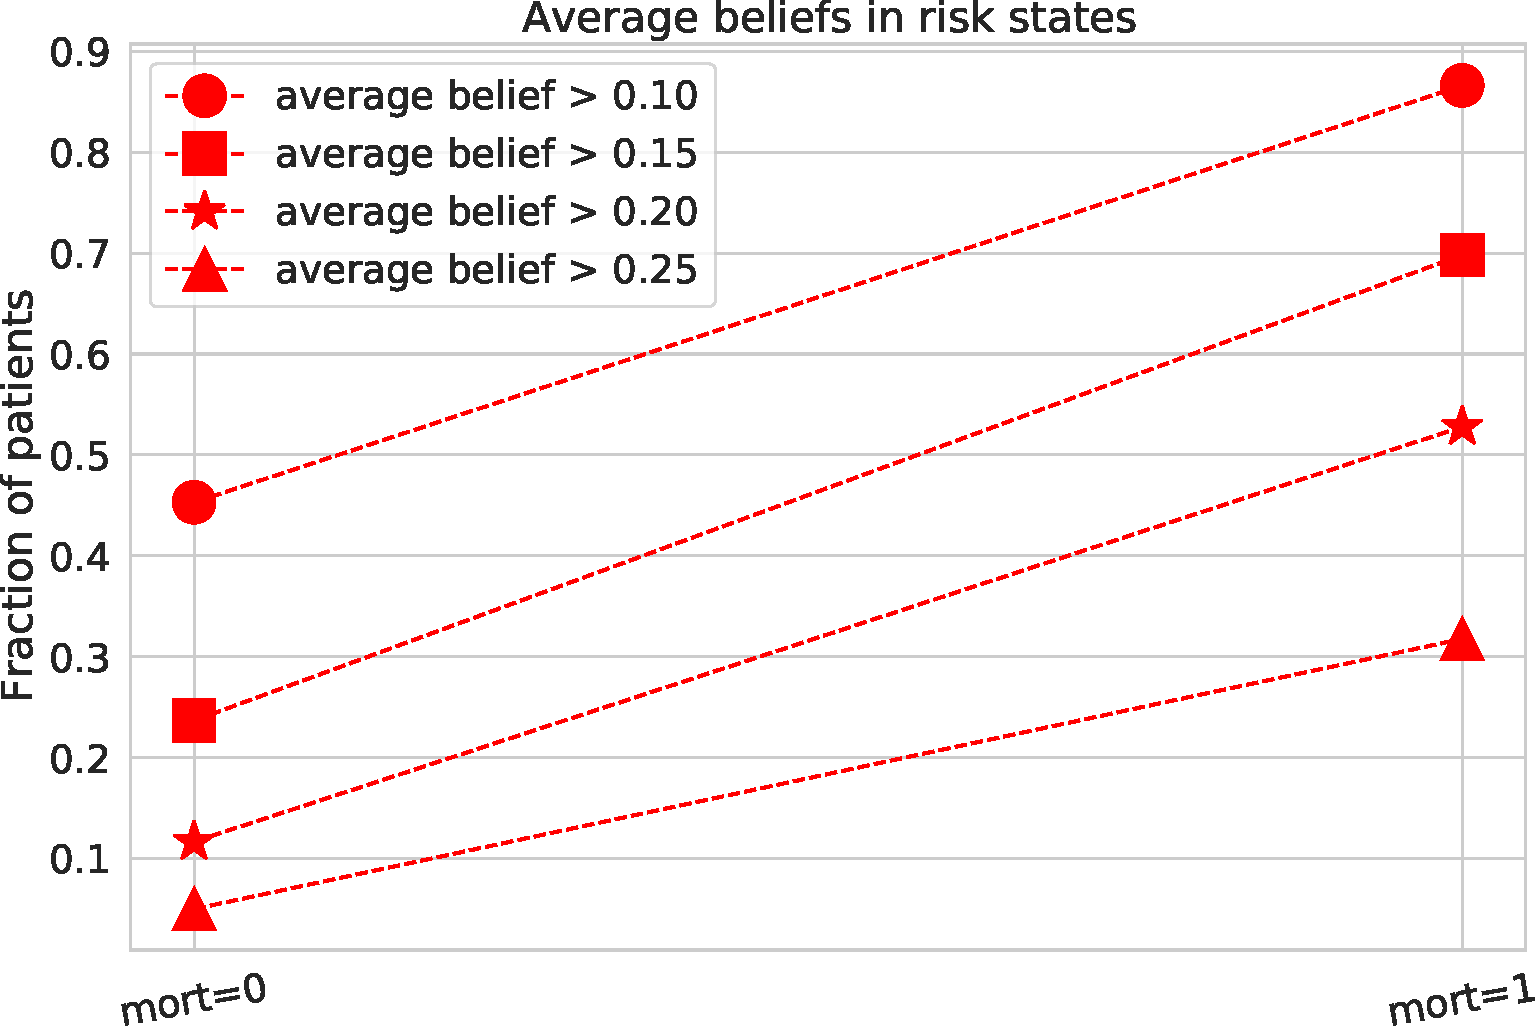
\includegraphics[width=0.5\textwidth]{content/chapters/semi_supervised_pchmm_missing_data/images/avg_beliefs_plots_for_mortality.pdf}
\end{tabular}
\caption[Interpretation of learned PC-HMM for mortality prediction]{
Interpretation of learned PC-HMM on eICU data.
\textbf{\textit{Top Left}}: Gaussian emission distributions of states and their $\eta_k$ (predictor weights).
The red and green states represent high risk (high $\eta_k$).
High risk states seem to represent populations with high heart rate and high creatinine levels (above 1.9mg/dL), which could indicate kidney problems~\citep{baha2021effect}.
\textbf{\textit{Top Right}}: For a patient labeled $y=1$ (who eventually dies), high heart rate and high creatinine are observed throughout the stay, and thus beliefs $b_t$ give highest probability to high risk states.
The probability of state $2$ (green) peak during segments of high creatinine and low oxygen saturation
\textbf{\textit{Bottom}}: We show the average beliefs (averaged over time) of normal patients and risk patients. Clearly, patients at risk spend more time in the risk state compared to the normal patients.
}%endcaption
\label{fig:interpretability_mortality}
\end{figure}